\textbf{(11.7) Пусть $P$ -- некоторое подмножество точек комплексной плоскости. Назовём точечным полем
для $P$ минимальное расширение $L \supset Q, L \subset C$, которое содержит обе координаты всех точек из $P$. Пусть
точка $z = x + y \cdot i$ получается при помощи операции пересечения прямых/окружностей из множества
точек $P$. Тогда $x, y$ лежат в расширении точечного поля $L$ для точек $P$ степени не больше, чем $2$.
Покажите это в случае, когда мы а) пересекаем две прямые; б) пересекаем прямую и окружность;
в) пересекаем две окружности.}

Пусть $P$ -- некоторое подмножество точек комплексной плоскости. Назовём точечным полем
для $P$ минимальное расширение $L \supset Q, L \subset C$, которое содержит обе координаты всех точек из $P$ (то есть, $\forall a = b + ic \in P: \ b \in L, c \in L$). Пусть
точка $z = x + y \cdot i$ получается при помощи операции пересечения прямых/окружностей из множества
точек $P$. Тогда $x, y$ лежат в расширении точечного поля $L$ для точек $P$ степени не больше, чем $2$.

а) Пусть мы получили точку $z$ как точку пересечения прямых через точки $z_1, z_2$ и $z_3, z_4$. Причем, $z_i = x_i + i \cdot y_i$. Дано: $x_1, x_2, x_3, x_4, y_1, y_2, y_3, y_4 \in L$.\\

\begin{minipage}{0.4\textwidth}
  \centering
  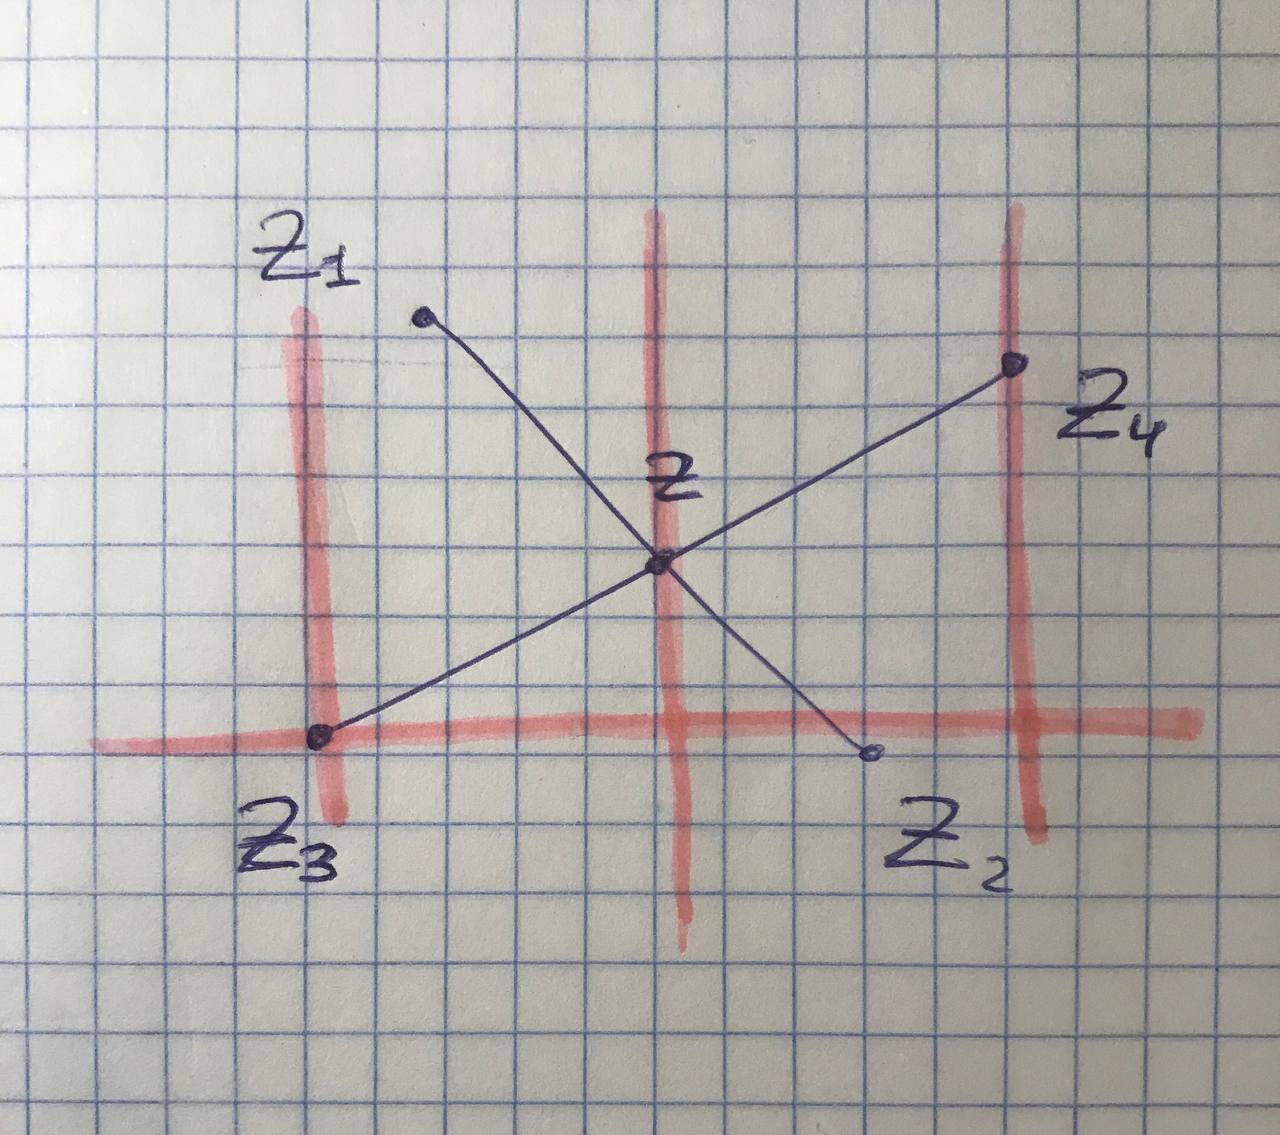
\includegraphics[width=0.7\linewidth]{sections/Ira/images/3-45_1.jpg}
\end{minipage}\\

В случае, когда прямые (или одна из них) параллельны осям координат, все просто. Рассмотрим самый содержательный вариант -- когда обе не параллельны, тогда верна система:

\begin{equation}
\begin{cases}
    \mathlarger{\frac{x - x_1}{x_2 - x_1} = \frac{y - y_1}{y_2 - y_1}} \\
    \\
    \mathlarger{\frac{x - x_3}{x_4 - x_3} = \frac{y - y_3}{y_4 - y_3}}
\end{cases}
\end{equation}

Из одного уравнения мы можем выразить $x$ и подставить в другое, получим, что $y$ линейно выражается через координаты известных точек. Тогда $x, y \in \mathbb{Q}(x_1, x_2, x_3, x_4, y_1, y_2, y_3, y_4) \Rightarrow x, y \in L$\\

б)  Пусть мы получили точку $z$ как точку пересечения прямой через точки $z_1, z_2$ и окружности с центром в точке $z_3$, проходящей через точку $z_4$. (Координаты так же лежат в $L$)\\

\begin{minipage}{0.4\textwidth}
  \centering
  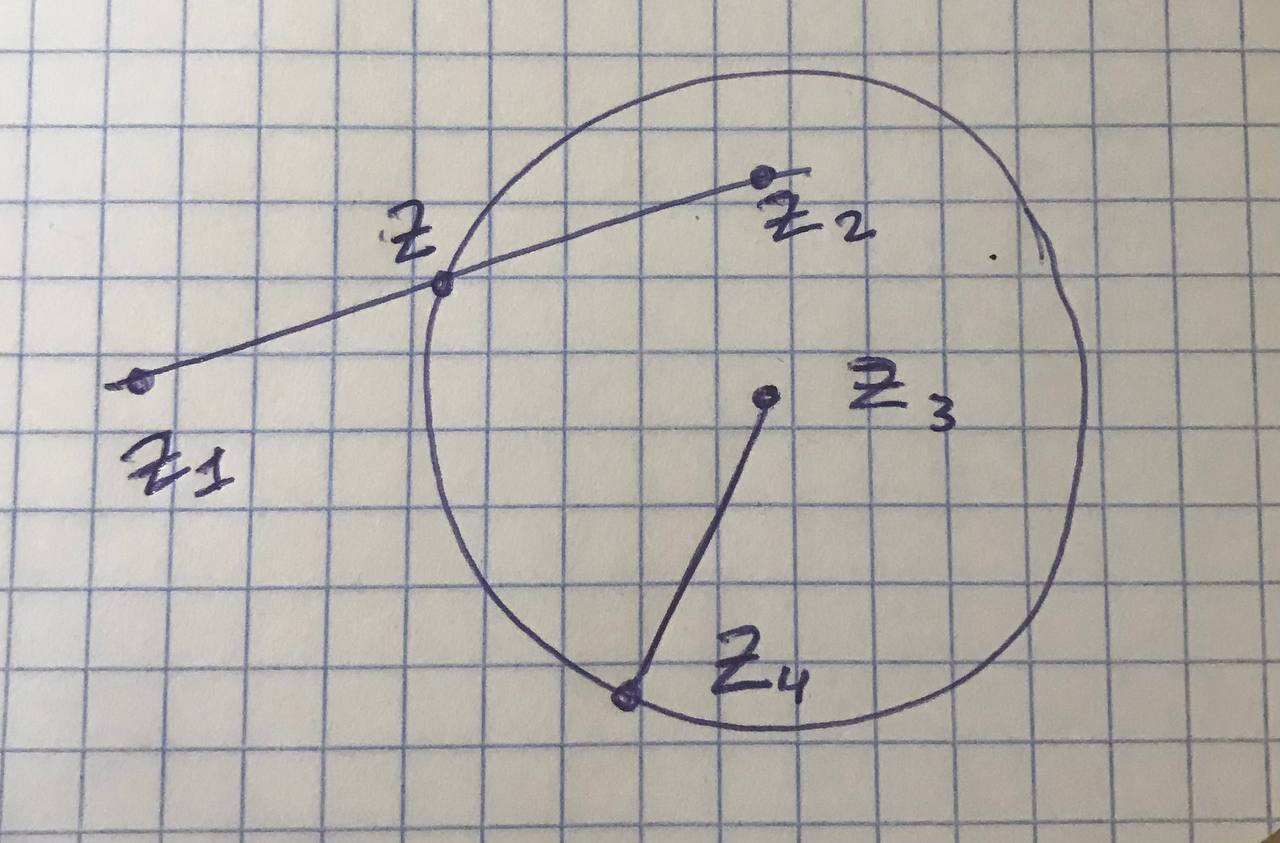
\includegraphics[width=0.8\linewidth]{sections/Ira/images/3-45_2.jpg}
\end{minipage}\\

Тогда получаем систему:

\begin{equation}
\begin{cases}
    \mathlarger{\frac{x - x_1}{x_2 - x_1} = \frac{y - y_1}{y_2 - y_1}} \\ \\
    (x-x_3)^2 + (y-y_3)^2 = (x_4 - x_3)^2 + (y_4 - y_3)^2
\end{cases}
\end{equation}

Из первого уравнения выразим $x$, подставим в уравнение окружности. Получим квадратное уравнение с $y$ и коэффициентами, выраженными через координаты известных точек. 

\textit{Замечание:} уравнение может получиться и вырожденным (отсюда и знак неравенства далее).

Поэтому $y \in K \supset L, [K:L] \leq 2$

в) В данном случае точка $z$ -- точка пересечения окружности с центром $z_1$ через точку $z_2$ и окружности с центром $z_3$ через точку $z_4$.

Система будет выглядеть так:

\begin{equation}
\begin{cases}
    (x-x_1)^2 + (y-y_1)^2 = (x_2 - x_1)^2 + (y_2 - y_1)^2 \\
    (x-x_3)^2 + (y-y_3)^2 = (x_4 - x_3)^2 + (y_4 - y_3)^2
\end{cases}
\end{equation}

Заметим, что если из первого уравнения вычесть второе, то $x^2, y^2$ сократятся, поэтому останется линейное уравнение, из которого можно так же выразить $x$ и подставить в одно из уравнений системы. Снова получим уравнение степени не более $2$, которое зависит только от $y$.

Аналогично предыдущему пункту $y \in K \supset L, [K:L] \leq 2$.
